\section{Performance Comparison with BlockSim}\label{sec:comparison}

This section presents a performance comparison between \iblock{} and BlockSim,
the open-source Python simulator already discussed in \secref{subsec:blocksim}
\cite{blocksim}.

A fair comparison is impossible as \iblock{} is a more comprehensive Bitcoin
simulator, while BlockSim only simulates basic block and transaction
propagation with limited statistical reporting. BlockSim offers two modes:
``Light'' and ``Full''. In ``Light'' mode, BlockSim prioritizes speed by
bypassing network propagation of transactions, adding them directly to blocks.
In ``Full'' mode, BlockSim includes a basic form of transaction propagation but
it really is just a propagation delay randomly extracted from a predefined
distribution. By contrast, \iblock{} utilizes \omnetpp's functionalities to
propagate transactions across the network, which causes the receiving node to
do some processing when receiving a transaction, such as verifying that the
transaction is not already in the mempool or in the blockchain or updating the
list of UTXOs in the wallet.

BlockSim ``Full'' mode encounters limitations with larger simulations, as it
fails to simulate beyond a few hours due to excessive memory usage. In a test
simulating a 12-hour scenario with 30 nodes, BlockSim ``Full'' was terminated
by the Linux's Out-Of-Memory Killer after exceeding 30 GB of virtual memory.
Consequently, BlockSim ``Light'' mode will be used for comparisons involving
simulations longer than a few hours.

The experiments in this section follow a consistent scenario setup: 30 nodes,
including 10 miners, generating 3 transactions per second globally. For
\iblock{}, the default statistics recording mode is enabled, and BlockSim's
statistics collection, which is always active, is used as is. Notably,
\iblock{} gathers a much broader range of statistics than BlockSim, which
focuses only on mined blocks and miners' revenues.

The objective of these comparisons is to demonstrate that \iblock{} can perform
simulations with greater detail than BlockSim ``Full'' while requiring less
resources.

\subsection{Comparison with BlockSim ``Light''}

The performance of \iblock{} was compared with BlockSim ``Light'' by running
both simulators in the proposed scenario for 2-day and 7-day simulated periods.
\figref{subfig:comparison-48h} presents the memory usage progression over the
2-day simulation, and \figref{subfig:comparison-168h} shows memory usage for
the 7-day simulation.

\begin{figure}[p]
	\centering
	\begin{subfigure}[b]{0.85\textwidth}
		\centering
		\includegraphics[width=\textwidth,trim={3.05cm 1.85cm 3.3cm
			2.5cm},clip]{blocksim-comp-48}
		\caption{2-day simulation.}\label{subfig:comparison-48h}
	\end{subfigure}
	\par\bigskip\medskip
	\begin{subfigure}[b]{0.85\textwidth}
		\centering
		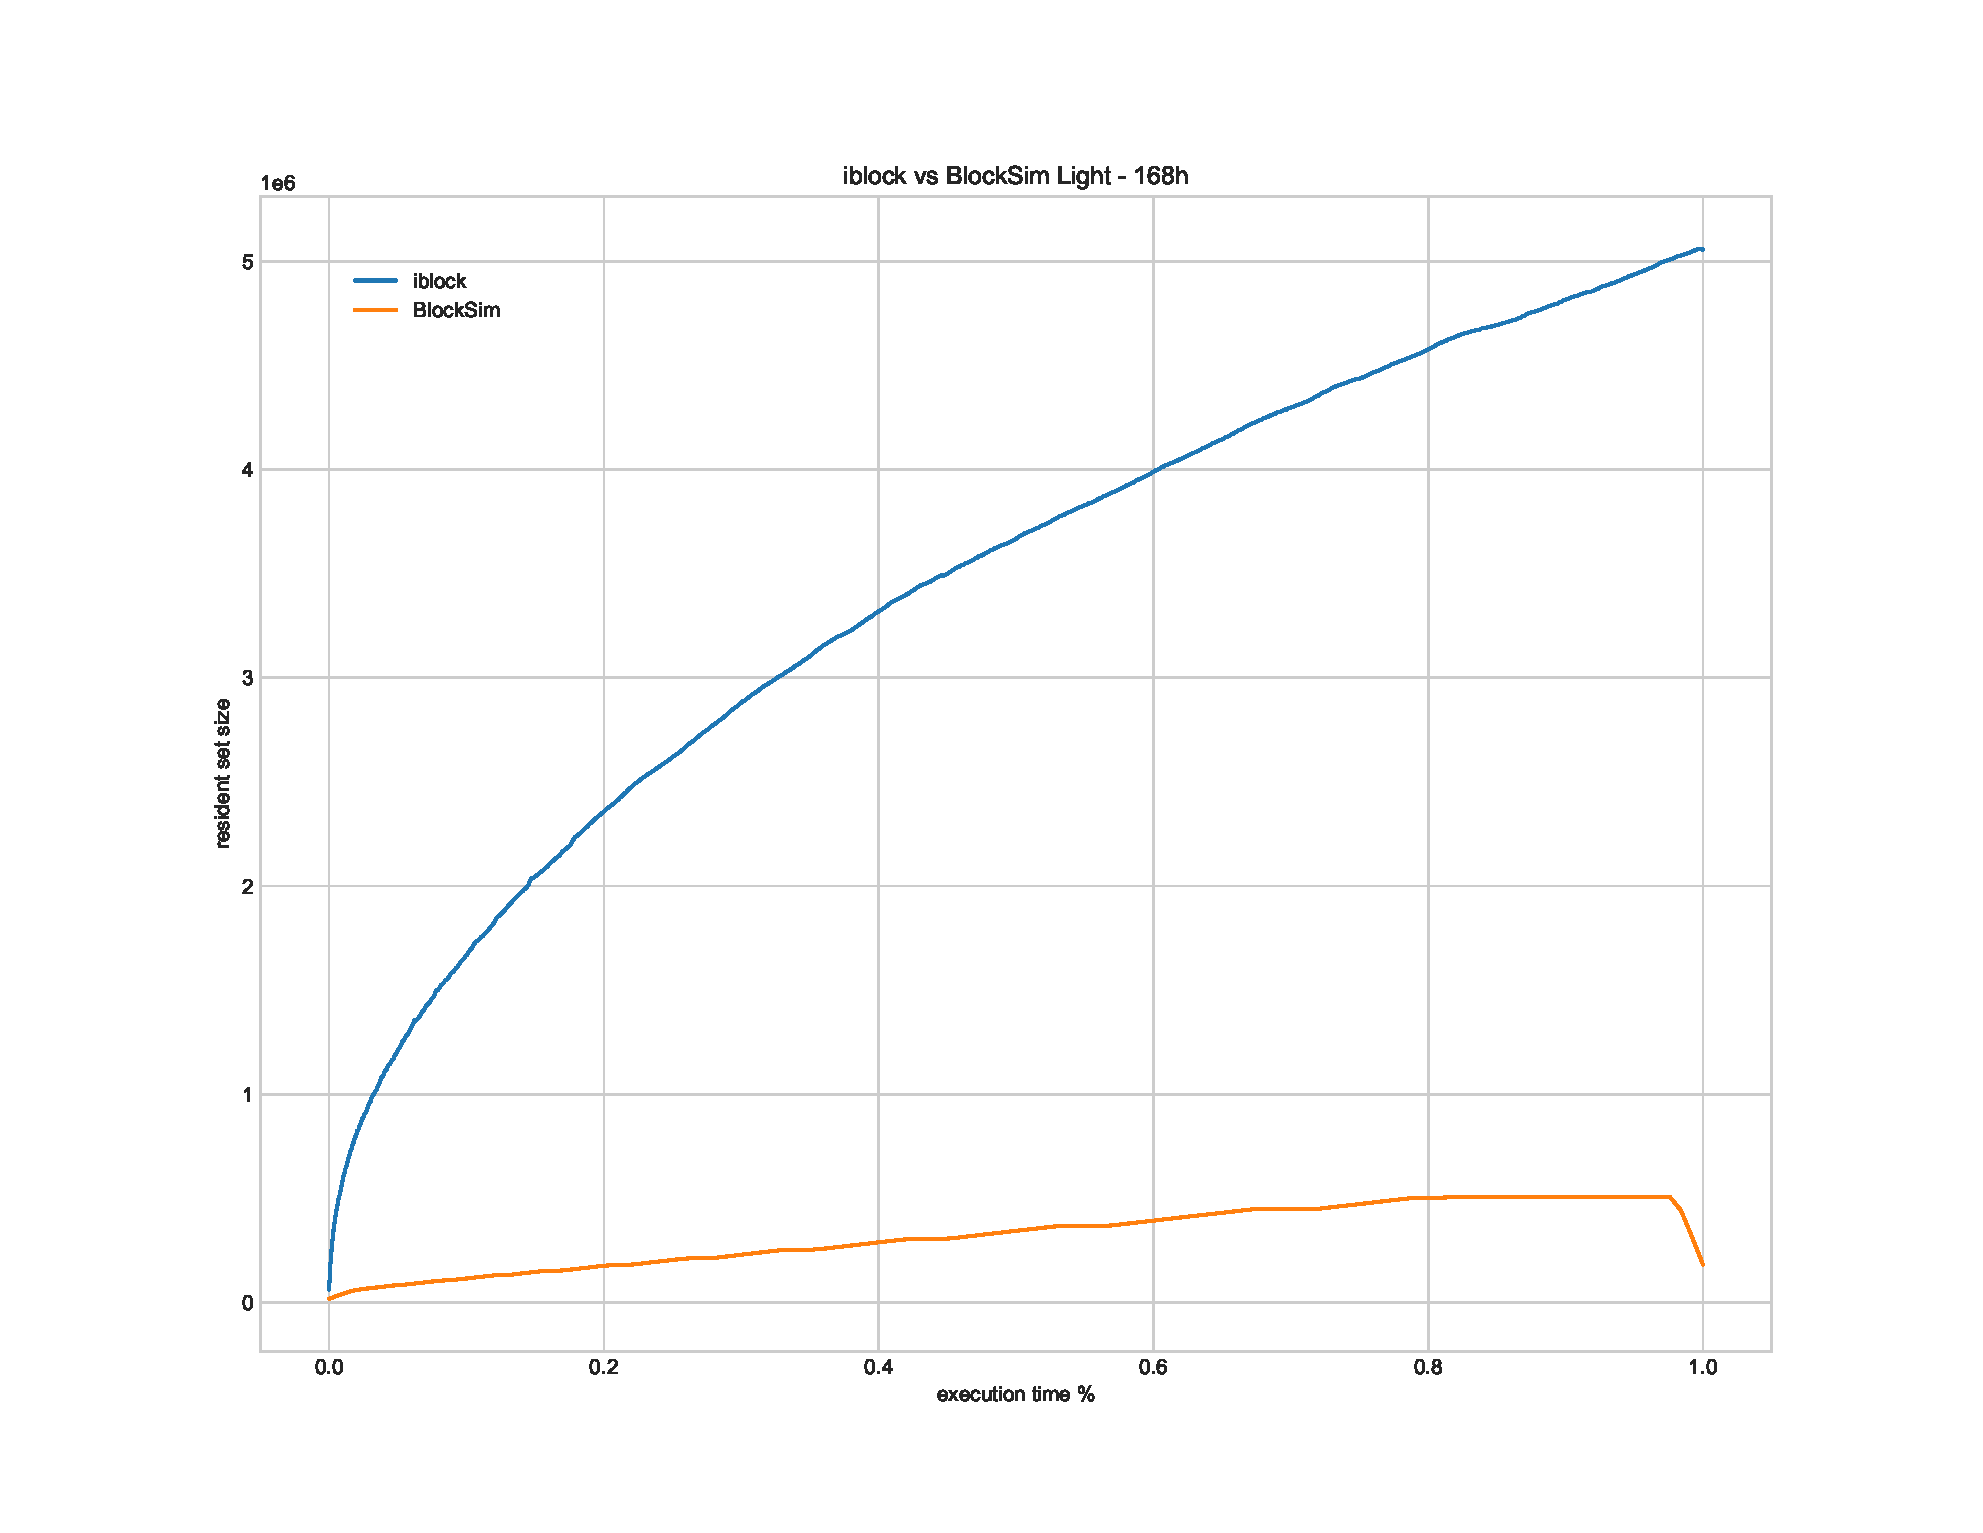
\includegraphics[width=\textwidth,trim={3.05cm 1.85cm 3.3cm
			2.5cm},clip]{blocksim-comp-168}
		\caption{7-day simulation.}\label{subfig:comparison-168h}
	\end{subfigure}
	\caption{Comparison of memory consumption over time between \iblock{}
	and BlockSim ``Light'' for 2 and 7 days of simulated
	time.}\label{fig:comparison-light}
\end{figure}

Regarding the execution time, \iblock{} completed the 2-day simulation in 7
minutes and 22 seconds, whereas BlockSim ``Light'' required only \(2.5\)
seconds. The 7-day simulation took 1 hour 40 minutes and 6 seconds with
\iblock{} and only \(8.2\) seconds with BlockSim ``Light''.

As expected, BlockSim ``Light'' is significantly faster than \iblock{}.
However, BlockSim ``Light'' does not meaningfully simulate network behavior, as
transactions are merely instances of a class added directly to blocks without
network propagation.

BlockSim ``Light'' also exhibits lower memory consumption than \iblock{} due to
its simplified structure. For instance, each node in \iblock{} maintains a
wallet that tracks Unspent Transaction Outputs (UTXOs), used to compute wallet
balances and create new transactions. By contrast, BlockSim only records a
sender and receiver in each transaction, while \iblock{} implements full
transaction details, including inputs and outputs, allowing for
multi-input/output transactions.

\subsection{Comparison with BlockSim ``Full''}

Since BlockSim ``Full'' attempts to generate all necessary transactions at the
outset, it usually exhausts memory before starting simulations that last beyond
a few hours of simulated time. Thus, the comparison between \iblock{} and
BlockSim ``Full'' is limited to simulations lasting up to six hours.

\figref{fig:comparison-full-memory} shows the total memory consumption for both
simulators over 1 to 6 hours simulations in the proposed scenario, while Table
\ref{tab:comparison-full-time} presents the comparison of their total execution
times --- the significant execution time difference between simulators makes
histogram-based comparisons impractical. Notice how BlockSim ``Full'' execution
time surpasses the simulated time for the 5-hour and 6-hour scenarios.

\begin{figure}[tbhp]
	\centering
	\includegraphics[width=\textwidth]{blocksim-comp-full}
	\caption{Comparison of memory consumption between \iblock{} and
	BlockSim ``Full'' over 1 to 6 hours of simulated
	time.}\label{fig:comparison-full-memory}
\end{figure}

\begin{table}[tbhp]
	\centering
	\begin{tabular}{|c|c|c|}
		\toprule
		Simulated Time & \iblock{} Exec\@. Time & BlockSim Exec\@. Time \\
		\midrule
		1 hour & 1s & 7m\,16s \\[6pt]
		2 hours & 2s & 28m\,8s \\[6pt]
		3 hours & 4s & 1h\,55m\,13s \\[6pt]
		4 hours & 5s & 3h\,13m\,56s \\[6pt]
		5 hours & 7s & 6h\,30m\,46s \\[6pt]
		6 hours & 10s & 7h\,16m\,59s \\
		\bottomrule
	\end{tabular}
	\caption{Execution time comparison between \iblock{} and BlockSim
	``Full''.}\label{tab:comparison-full-time}
\end{table}

Overall, \iblock{} demonstrates significantly better performance than BlockSim
``Full'' in terms of both memory consumption and execution time, even while
running more detailed simulations. In terms of performance, \iblock{} sits
between BlockSim ``Light'' and BlockSim ``Full'', but it achieves a level of
network simulation detail that even BlockSim ``Full'' cannot match. \iblock{}
collects detailed statistics per node and network-wide, enabling investigation
into various simulation properties. In contrast, BlockSim only gathers basic
aggregated statistics on blocks and miners' revenues.
